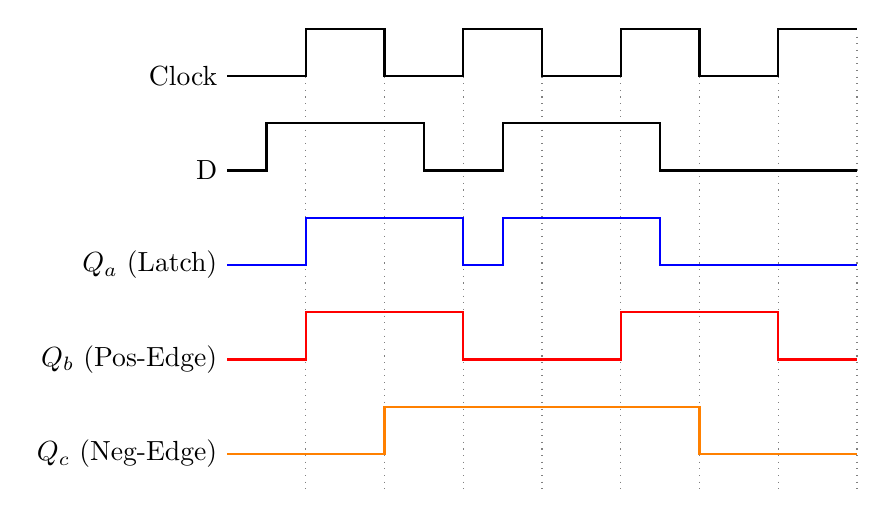
\begin{tikzpicture}
    % Define coordinates
    \def\tick{0.2}
    \def\h{0.6} % Height of logic high
    \def\sep{-1.2} % Separation between signals

    % Labels
    \node[anchor=east] at (0, 0) {Clock};
    \node[anchor=east] at (0, \sep) {D};
    \node[anchor=east] at (0, 2*\sep) {$Q_a$ (Latch)};
    \node[anchor=east] at (0, 3*\sep) {$Q_b$ (Pos-Edge)};
    \node[anchor=east] at (0, 4*\sep) {$Q_c$ (Neg-Edge)};

    % Draw Axes/Grid lines
    \foreach \x in {1,2,...,8} {
        \draw[dotted, gray] (\x, 0.5) -- (\x, 4*\sep - 0.5);
    }

    % Clock Signal (Period = 2 units)
    % 0-1 Low, 1-2 High...
    \draw[thick] (0,0) -- (1,0) -- (1,\h) -- (2,\h) -- (2,0) -- (3,0) -- (3,\h) -- (4,\h) -- (4,0) -- (5,0) -- (5,\h) -- (6,\h) -- (6,0) -- (7,0) -- (7,\h) -- (8,\h);

    % D Input (Arbitrary)
    % 0-0.5: 0
    % 0.5-2.5: 1
    % 2.5-3.5: 0
    % 3.5-5.5: 1
    % 5.5-8.0: 0
    \draw[thick] (0, \sep) -- (0.5, \sep) -- (0.5, \sep+\h) -- (2.5, \sep+\h) -- (2.5, \sep) -- (3.5, \sep) -- (3.5, \sep+\h) -- (5.5, \sep+\h) -- (5.5, \sep) -- (8, \sep);

    % Qa (Gated D Latch) - Transparent when Clk=1
    \draw[thick, blue] (0, 2*\sep) 
        -- (1, 2*\sep)       % Hold 0
        -- (1, 2*\sep+\h)    % @1.0 Clk->1, D=1 -> 1
        -- (3, 2*\sep+\h)    % Hold 1 until 3.0
        -- (3, 2*\sep)       % @3.0 become 0
        -- (3.5, 2*\sep)     % Follow 0
        -- (3.5, 2*\sep+\h)  % @3.5 D->1, Clk=1 -> Follow 1
        -- (5.5, 2*\sep+\h)  % Hold/Follow 1
        -- (5.5, 2*\sep)     % @5.5 Follow 0
        -- (8, 2*\sep);      % 0

    % Qb (Pos-Edge D FF) - Sample D at Rising Edge (1, 3, 5, 7)
    \draw[thick, red] (0, 3*\sep) 
        -- (1, 3*\sep)    % Init 0
        -- (1, 3*\sep+\h) % @1 D=1 -> 1
        -- (3, 3*\sep+\h) % Hold
        -- (3, 3*\sep)    % @3 D=0 -> 0
        -- (5, 3*\sep)    % Hold
        -- (5, 3*\sep+\h) % @5 D=1 -> 1
        -- (7, 3*\sep+\h) % Hold
        -- (7, 3*\sep)    % @7 D=0 -> 0
        -- (8, 3*\sep);

    % Qc (Neg-Edge D FF) - Sample D at Falling Edge (2, 4, 6)
    \draw[thick, orange] (0, 4*\sep) 
        -- (2, 4*\sep)    % Init 0
        -- (2, 4*\sep+\h) % @2 D=1 -> 1
        -- (6, 4*\sep+\h) % Hold
        -- (6, 4*\sep)    % @6 D=0 -> 0
        -- (8, 4*\sep);

\end{tikzpicture}
